\chapter{Results}

\section{Measures of transport error}
[[[The area containing the ensemble of parcels should grow as $t^{1/2}$, so should the RMSE as well? 
The errors of neighboring points are highly correlated, so the RMSE shows the general $t^{1/2}$ trend, but there's a lot of noise based on idiosyncrasies of the flow in that region. 
Maybe plot average RSME of all experiment locations over time?

The AHTD and RMSE are analogous to standard deviation.
We discussed finding error bars on the AHTD and RHTD values by calculating them for ensembles started nearby: 
shifted a degree in every direction, for example. 
I could find the mean and standard deviation of AHTD and RHTD for the 3x3 grid of ensembles created by shifting the starting ensemble north/south/east/west.
Are the shifted ensembles still in the same flow regime? How generalizable are error bars on AHTD and RHTD to the whole model, then?

Perhaps AHTD and RHTD are better measures for a larger grid, to get a measure of trajectory error for the whole model. 
In that case, instead of the 3x3 grid of trajectory ensembles, I could try a mesh of trajectory starting points over the whole globe.
6 degree spacing or so. 
The AHTD and RHTD would be a "whole model" reference, to which the AHTD and RHTD for more specific ensemble launch locations (like Boston) could be compared.]]]

\begin{table}
    \centering
    \caption{Measures of transport error after 213 hours.}    
    \begin{tabular}{ l l l r r }
        \hline
        \hline
        			&				&				& 	\multicolumn{2}{c}{Location} \\
	\cline{4-5}
        Statistic 	& Model 			& Reference 		& Boston 		& Barau		\\
        \hline
        RMSE	& kinematic 		& mean trajectory	& 1,444 km	& 1,342 km	\\
        		 	& dynamic 		& mean trajectory	& 2,800 km	& 5,607 km	\\
			& HYSPLIT 3D 		& mean trajectory	& 5,630 km	& 2,270 km	\\
        		 	& HYSPLIT isobaric 	& mean trajectory	& 4,740 km	& 1,260 km	\\
        AHTD 	& kinematic		& HYSPLIT 3D		& 2,160 km	& 1,130 km	\\
        		 	& dynamic			& HYSPLIT 3D 		& 1,940 km	& 1,630 km	\\
        		 	& kinematic		& HYSPLIT isobaric  & 1,270 km	& 1,300 km	\\
        		 	& dynamic			& HYSPLIT isobaric  & 1,200 km	& 1,730 km	\\
			& HYSPLIT isobaric	& HYSPLIT 3D 		& 1,930 km	& 588 km		\\
        RHTD 	& kinematic		& HYSPLIT 3D		& 0.48		& 0.92		\\
        		 	& dynamic			& HYSPLIT 3D 		& 0.43		& 1.30		\\
        		 	& kinematic		& HYSPLIT isobaric  & 0.23		& 1.20		\\
        		 	& dynamic			& HYSPLIT isobaric  & 0.22		& 1.60		\\
			& HYSPLIT isobaric	& HYSPLIT 3D 		& 0.012		& 0.019		\\	
        \hline
    \end{tabular}
\end{table}

\begin{figure}
    \centering
    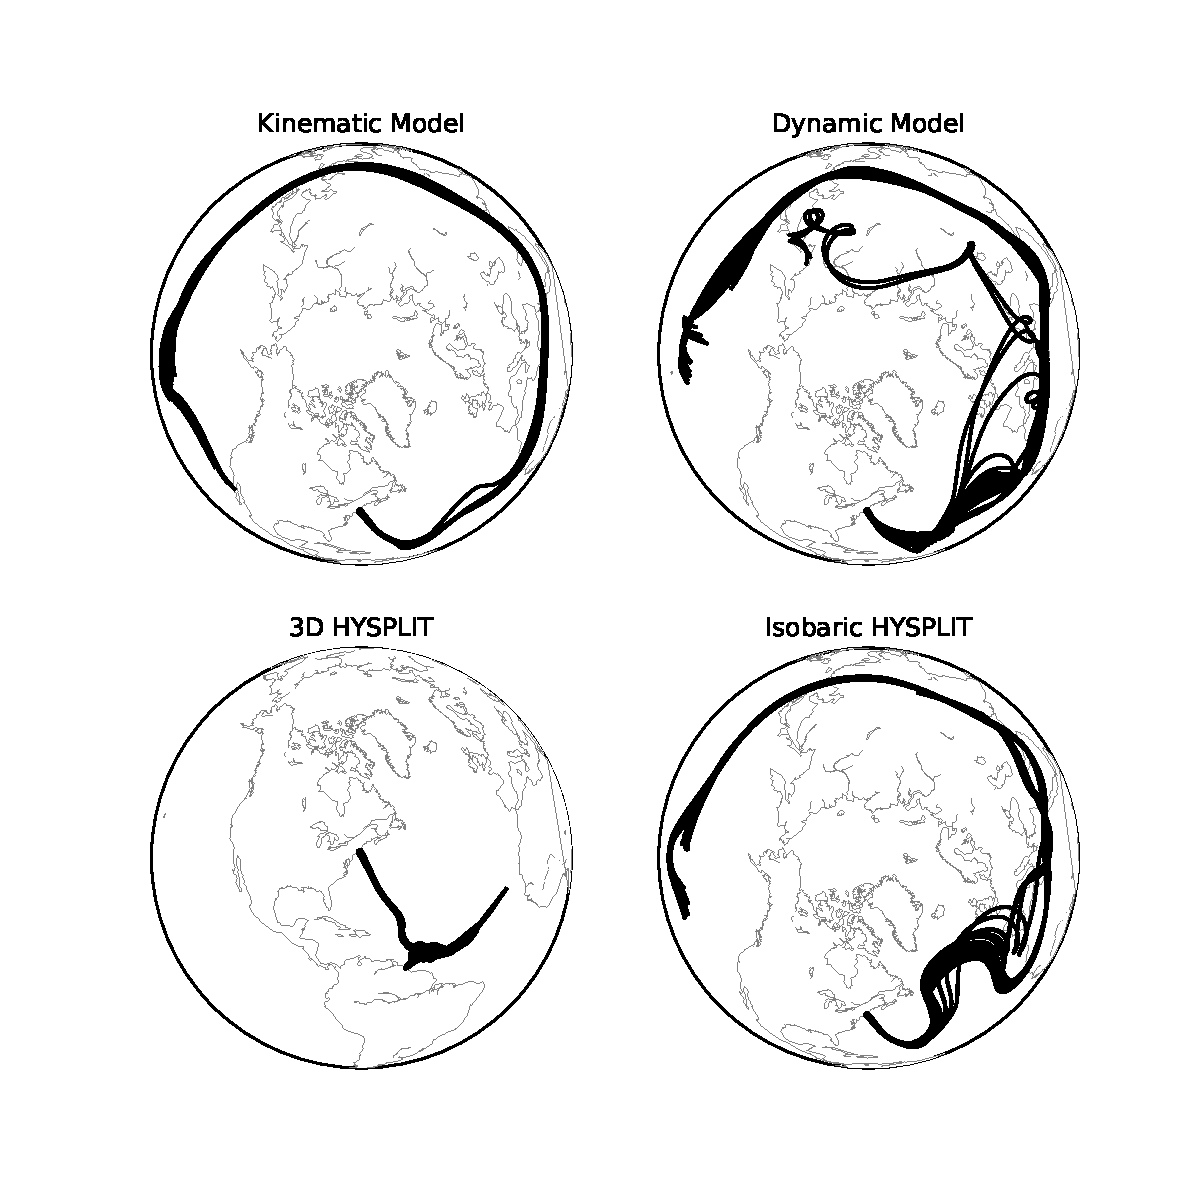
\includegraphics[width=\textwidth]{four_ortho.pdf}
    \caption{Trajectories for both models with reference trajectories for parcels launched from the 5x5 grid between 41$^\circ$N, 72$^\circ$W and 42$^\circ$N, 71$^\circ$W. }
\end{figure}